\subsection{Généralités}

Dans cette section, nous introduisant les \glspl{mlp},
l'architecture neuronale la plus simple et la plus utilisée.
Il s'agit d'une simple composition de couches affines avec des activations non affines 
(voire Définition~\ref{def. mlp}).


\begin{definition}[\Gls{mlp}~\cite{Mukherjee_2021}]\ \\
    \label{def. mlp}
    Soient \(k, w_0, w_1, \cdots, w_{k+1}\in\naturals\), 
    un réseau de neurones feed-forward de profondeur \(k+1\), à \(w_0\) entrées et \(w_{k+1}\) sorties, 
    est défini par une fonction :
    \begin{equation}
        \label{eq. mlp}
        \left\{
        \begin{array}{l}
            \reals^{w_0} \to \reals^{w_{k+1}}\\
            x\mapsto
            \phi_{k+1} \circ A_{k+1} \circ \phi_k \circ A_k \circ \cdots \circ \phi_1 \circ A_1(x)
        \end{array}
        \right.
    \end{equation}
    Où les \(A_i\) sont des fonctions affines \(\reals^{w_{i-1}}\to\reals^{w_i}\) 
    et les \(\phi_i\) sont des fonctions quelconques, typiquement non affines
    \(\reals^{w_i}\to\reals^{w_i}\), dites \emph{d'activations}.
    La fonction \(\phi_i\circ A_i\) est appelée la \(i^{\, \mathrm{eme}}\) couche du réseau.
\end{definition}

Un tel réseau de neurones est souvent représenté par 
un graphe orienté acyclique \((k+1)-\)partie  appelé son ``architecture sous-jacente''~\parencite{Kearns_Vazirani_1994}. 
La Figure~\ref{fig. mlp} illustre l'architecture d'un \gls{mlp} de profondeur 4
avec \((w_0, w_1, w_2, w_3, w_4) = (4, 5, 7, 5, 4)\).


\begin{figure}[hbt]
    \begin{center}
        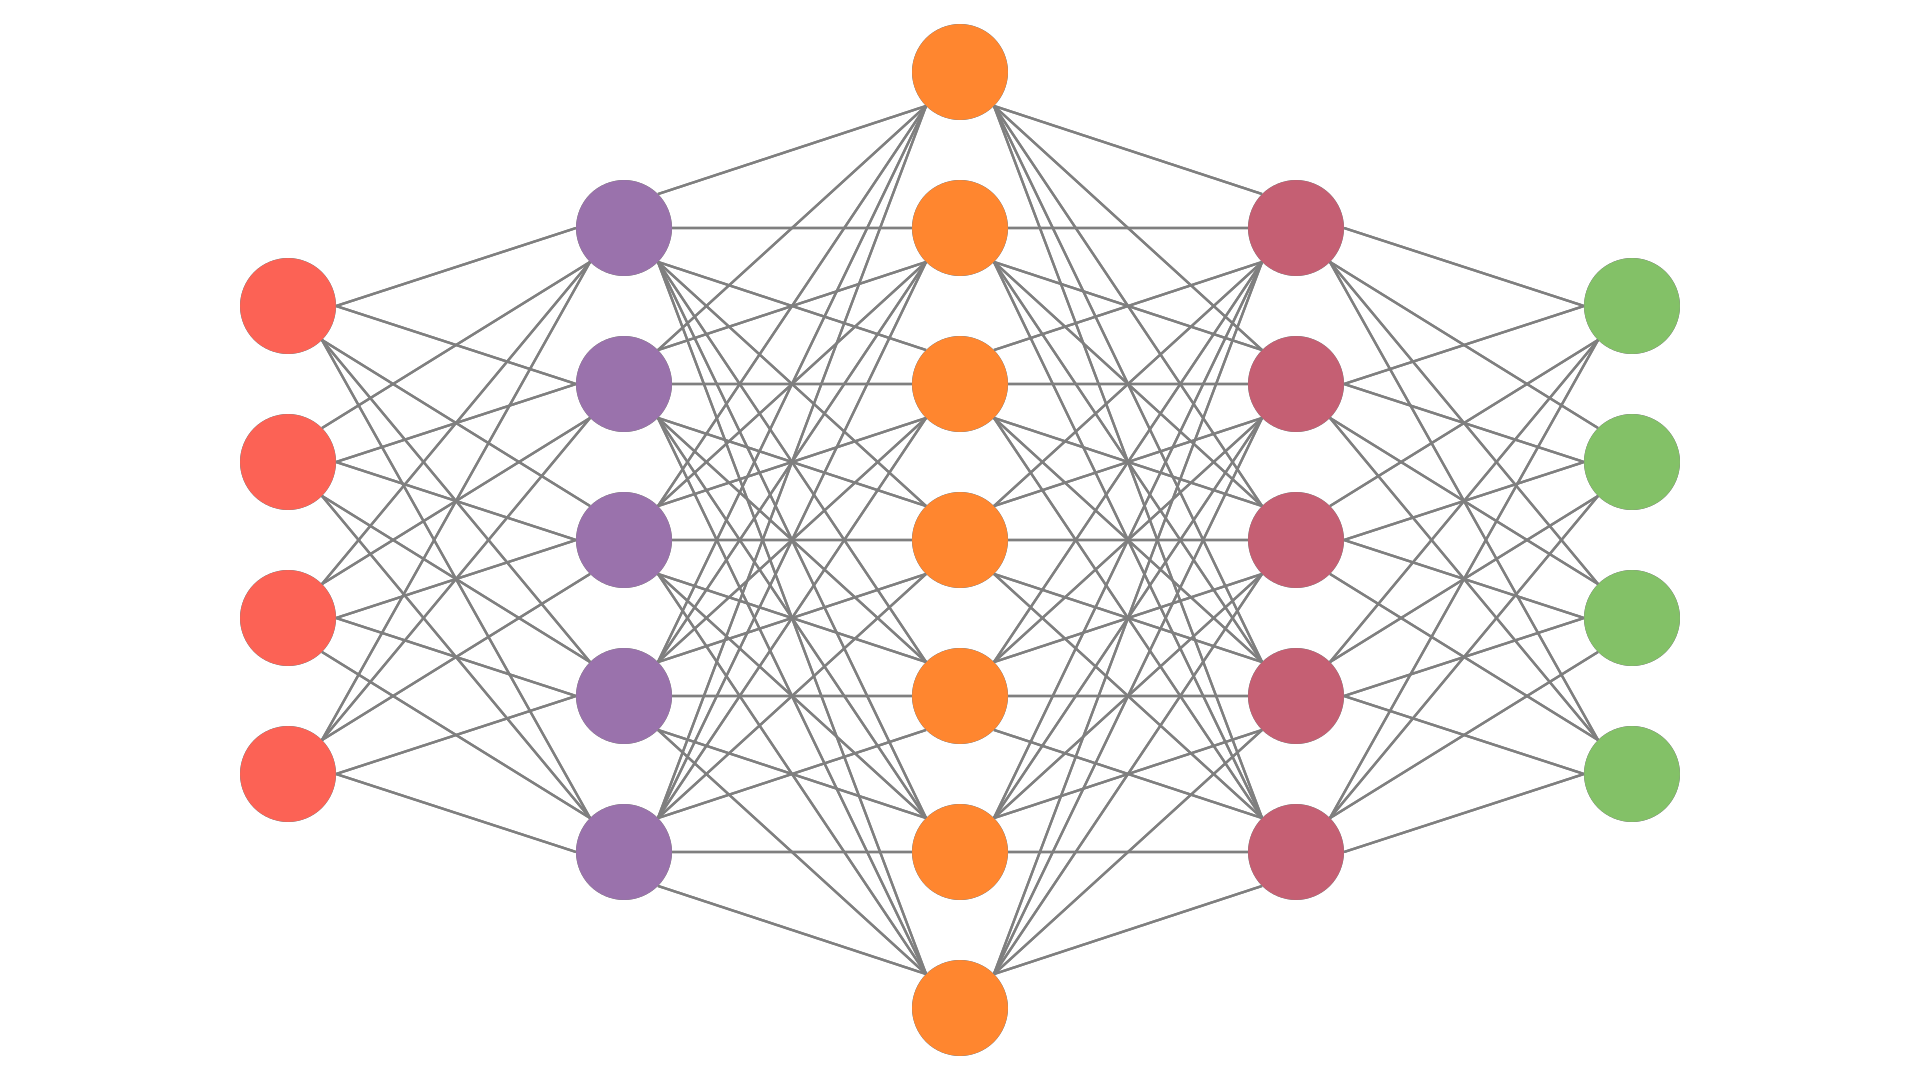
\includegraphics[width=10cm]{mlp.png}
    \end{center}
    \caption{Architecture sous-jacente d'un \glsfmtshort{mlp} de profondeur 3.}
    \label{fig. mlp}
\end{figure}

Deux \glspl{mlp} peuvent avoir la même architecture sous-jacente,
en effet, cette dernière ne dépend que des dimensions de leurs couches respectives.
De ce fait, une méthode de trouver pour une architecture et une fonction cible données 
le meilleur \gls{mlp} est nécessaire.

Pour ce faire, nous exploitons le fait que 
les \(A_i\) soient des applications affines sur des espaces de dimensions finies.
Nous pouvons donc les écrire comme combinaisons de produits matriciels et de translations.
Le problème se réduit donc à régler \footnote{En \gls{ml}, le terme ``entraîner'' est plutôt utilisé.}
les paramètres des matrices en question. 
Cela nécessite une façon de quantifier la qualité d'approximation d'une fonction \(f\) par une autre \(\hat{f}\).
L'analyse fonctionnelle nous en donne plusieurs, les~\cref{eq. l1-norm,eq. l2-norm}
sont deux exemples récurrents de fonctions dites \emph{de perte}.

\begin{equation}
    \label{eq. l1-norm}
    L_1(f, \hat{f}) = \int \left\|f - \hat{f}\right\|
\end{equation}

\begin{equation}
    \label{eq. l2-norm}
    L_2(f, \hat{f}) = \int \left\|f - \hat{f}\right\|^2
\end{equation}

Ayant fixé une fonction de perte \(L\), l'entraînement revient à un problème d'optimisation.
Dans le cas particulier où \(L\) est différentiable, 
l'algorithme du gradient peut être utilisé pour trouver un minimum local.
Les gradients sont calculés en utilisant une méthode de dérivation automatique comme la rétro-propagation.
